
\thispagestyle{empty}
\begin{tikzpicture}[overlay]

\draw (7,-23) node {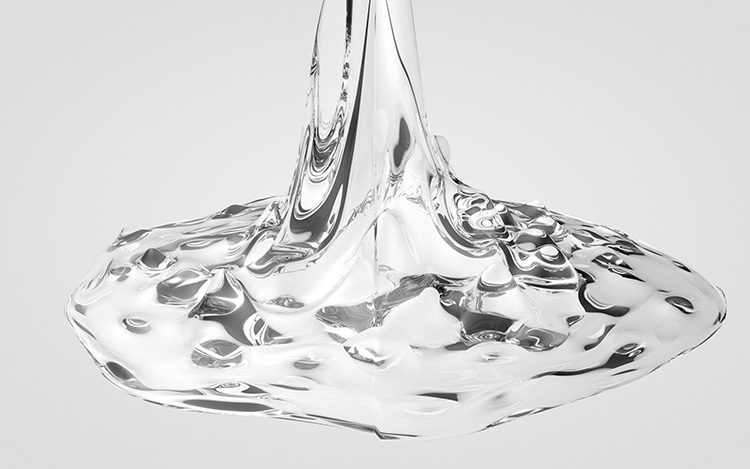
\includegraphics[origin=c,angle=90,width=21.5cm]{images/fondo2.jpg}};
\draw (7,-1) node {\fontsize{100}{100}\selectfont \color{black}\shadowtext{\textbf{MECÁNICA}}};
\draw (7,-4) node {\color{black}\fontsize{70}{80}\selectfont \textbf{de los FLUÍDOS}};
\draw (17,-27.5) node [above left]{\fontsize{25}{25}\color{black}\sffamily \shadowtext{\textbf{FERREYRA G.}}};
\draw (7,-6) node [below]{\fontsize{30}{30}\color{purple}\sffamily \shadowtext{\textbf{GUÍA de TRABAJOS PRÁCTICOS}}};
\end{tikzpicture}

%\maketitle